\documentclass[11pt]{article}
\usepackage{amsmath,amssymb}
\usepackage[makeroom]{cancel}
\usepackage{graphicx}
\usepackage{array}
\usepackage{changes}
\usepackage{natbib}
\graphicspath{ ../figs/}
\usepackage[margin=1in]{geometry}
\usepackage[parfill]{parskip}  
\title{Southwest US drought dynamics \large \\}
\author{Daniel Kennedy - djk2120@ucar.edu \\ Isla Simpson }

\begin{document}
\maketitle

\section{Introduction}

\begin{itemize}
    \item SWUS experienced a megadrought, and 2020 was the driest year on record.
    \item The 2020 drought was associated with xyz
    \item Climate change is not understood to have greatly exacerbated the 2020 drought.
    \item Whether average precipitation is projected to increase, decrease, or remain the same varies among climate models
    \item CESM2 projects that average precipitation will stay the same
    \item The statistics of determining whether extreme events are getting more extreme is more tenuous given the smaller sample size.
\end{itemize}


\begin{figure}[h]
\centering
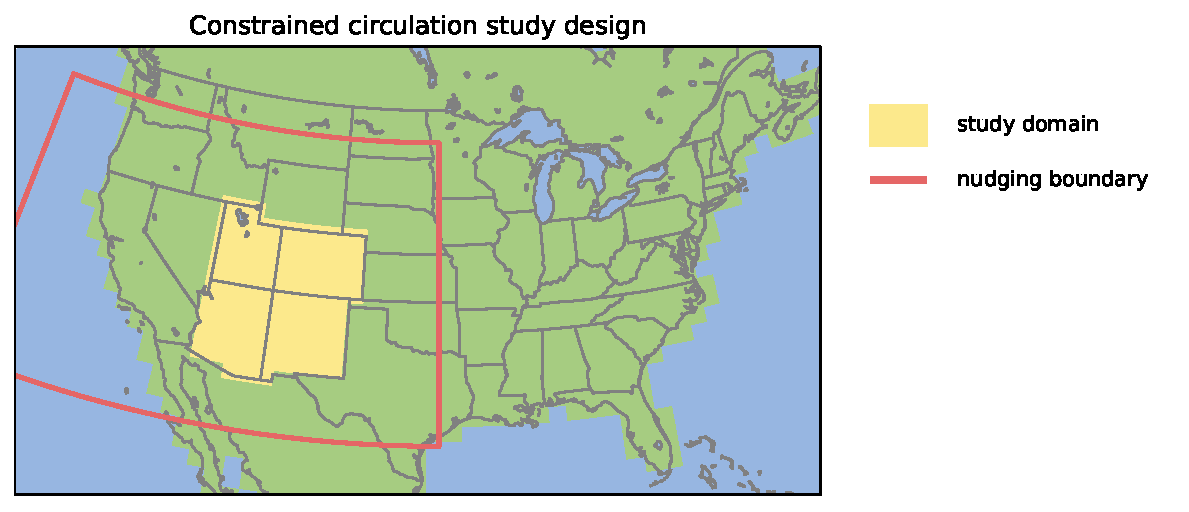
\includegraphics[width=40pc]{figs/domain.pdf}
\caption{Map of our study domain (yellow) and the nudging box (red).}
\label{fig:domain}
\end{figure}


\newpage

\begin{figure}[h]
\centering
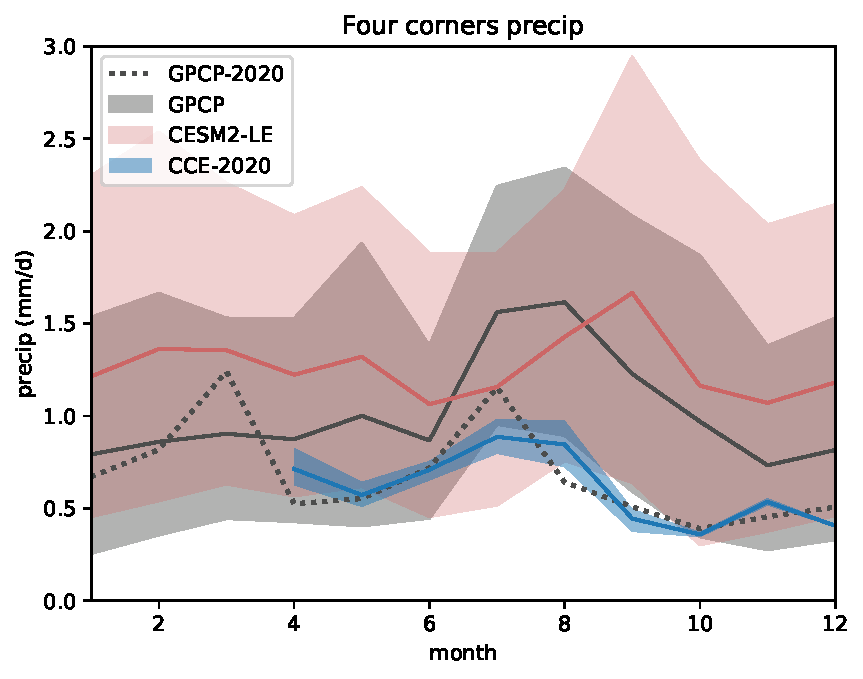
\includegraphics[width=40pc]{figs/main/precip.pdf}
\caption{Precip in the four corners.}
\label{fig:precip}
\end{figure}


\newpage
\begin{figure}[h]
\centering
\includegraphics[width=40pc]{figs/main/s}
\caption{Precip in the four corners.}
\label{fig:precip}
\end{figure}



Drought in the large ensemble:
\begin{itemize}
    \item CESM2 does not have a very strong NAM, and its timing is late, peaking in September.
    \item September also features the largest precipitation variance.
    \item September precipitation tends to exceed evapotranspiration, implying moisture convergence to the region. 
    \item Soil moisture initialization is not a strong control on JAS precip.
    
    
\end{itemize}


\bibliographystyle{abbrvnat}
\nocite{*}
\bibliography{refs/all}
\end{document}




